\section{Datasets and Models}
\label{sec:datasets_and_models}
This section details the datasets and models that form the basis of our mapping framework. We first introduce the simulated lunar dataset used for evaluation. Following this, we provide a comprehensive overview of various methods for two key perception tasks: dense depth estimation—-from both monocular and stereo inputs—-and semantic segmentation. The primary objective is to benchmark these models to characterize their performance within a lunar context and determine their suitability for the downstream task of real-time 3D reconstruction. Finally, we describe the fundamentals of 3D Gaussian Splatting, the scene representation used in our mapping pipeline.

\subsection{Dataset}
% \item \textbf{LuSNAR Dataset}~\cite{liu_lusnarlunar_2024}. 
We use the Lunar Segmentation, Navigation, and Reconstruction (LuSNAR) dataset, a comprehensive lunar benchmark dataset designed for evaluating autonomous perception and navigation systems~\cite{liu_lusnarlunar_2024}. It contains high-resolution stereo image pairs, semantic labels, dense depth maps, LiDAR point clouds, and rover position data. The dataset consists of 9 simulated lunar scenes created using Unreal Engine, each varying in terrain features and object density. These scenes are designed to represent different lunar surface conditions, from flat plains to cratered regions with varying rock distributions. The dataset enables the evaluation of key perception tasks, including semantic segmentation, 3D reconstruction, and autonomous navigation, making it a valuable resource for testing and validating lunar surface algorithms. However, it has some limitations: it does not provide full 3D geometry information, lacks closed-loop simulation capabilities, and has limited control over illumination conditions.
We are currently working on extending this study to include other datasets.

% \begin{itemize}
% \item \textbf{Open3D Environment}.
%       We developed a synthetic environment using Open3D \cite{zhou_open3d_2018} to generate lunar terrain with configurable elevation profiles and rock distributions, as illustrated in \cref{fig:sample_open3d}. This simulation environment provides several key capabilities: (1) high-fidelity RGB image rendering with precise ground truth depth maps and terrain geometry, (2) fine-grained control over rock placement, size distribution, and terrain features for systematic testing, and (3) flexible camera and lighting parameterization to simulate various operational conditions. However, the current implementation has limitations in simulating realistic rover dynamics and image quality. The physics simulation lacks accurate wheel-terrain interaction modeling, and the rendering pipeline does not fully capture the complex lighting conditions and sensor noise characteristics of actual lunar environments. These limitations affect the realism of the generated data and may impact the generalization of algorithms trained on this synthetic data to real-world scenarios. Despite these constraints, this controlled environment enables rapid prototyping and validation of perception algorithms under known ground truth conditions.


% 	\item \textbf{LAC Environment}~\cite{jhuapl_lunar_nodate}. The Lunar Autonomy Challenge (LAC) is a competition hosted by NASA, The Johns Hopkins University (JHU) Applied Physics Laboratory (APL), Caterpillar Inc., and Embodied AI. It provides a high-fidelity simulation environment with the most realistic representation of lunar conditions among our datasets, with high-fidelity rover dynamics including wheel-terrain interaction where wheels sink 2-3cm into the regolith and leave visible tracks. The simulation includes 8 cameras and an inertial measurement unit (IMU) sensor suite, enabling closed-loop simulations where we can directly control the rover's motion. However, it has several limitations: the available terrain area is restricted, illumination conditions are fixed, rock distributions cannot be modified, and it does not provide depth maps - instead having estimates based on the elevation field that do not include rocks or the lander. This limitation was one of the key motivations for developing our custom Open3D environment. The segmentation and depth estimation methods developed in this work contributed to winning the challenge, demonstrating their effectiveness for lunar surface navigation and mapping~\cite{noauthor_top_2025}.
% \end{itemize}

\subsection{Stereo Depth Estimation}
We evaluate the following stereo depth estimation models:
\label{sec:stereo_depth_estimation}
\begin{itemize}
	\item \textbf{Block Matching (BM)}: Computes disparity by comparing fixed-size image patches along epipolar lines using a cost function, such as Sum of Absolute Differences (SAD). Its performance is limited in textureless regions and under non-ideal illumination.

	\item \textbf{Semi-Global Matching (SGM)}~\cite{hirschmuller_stereo_2008}: Aggregates matching costs along multiple 1D paths across the image to approximate a 2D global smoothness constraint. This approach combines the efficiency of local methods with improved performance in low-texture areas.

	\item \textbf{RAFT-Stereo}~\cite{lipson_raft-stereo_2021}: Adapts the RAFT architecture from optical flow by constructing a 3D correlation volume of all disparities at all pixels. A recurrent, GRU-based unit then iteratively updates a high-resolution disparity field from this volume.

	\item \textbf{CREStereo}~\cite{li_practical_2022}: A cascaded recurrent network that operates in a coarse-to-fine manner. It uses recurrent refinement units at each stage and an adaptive group correlation layer to handle large displacements between stereo images.
\end{itemize}

\begin{figure}[t]
	\centering
	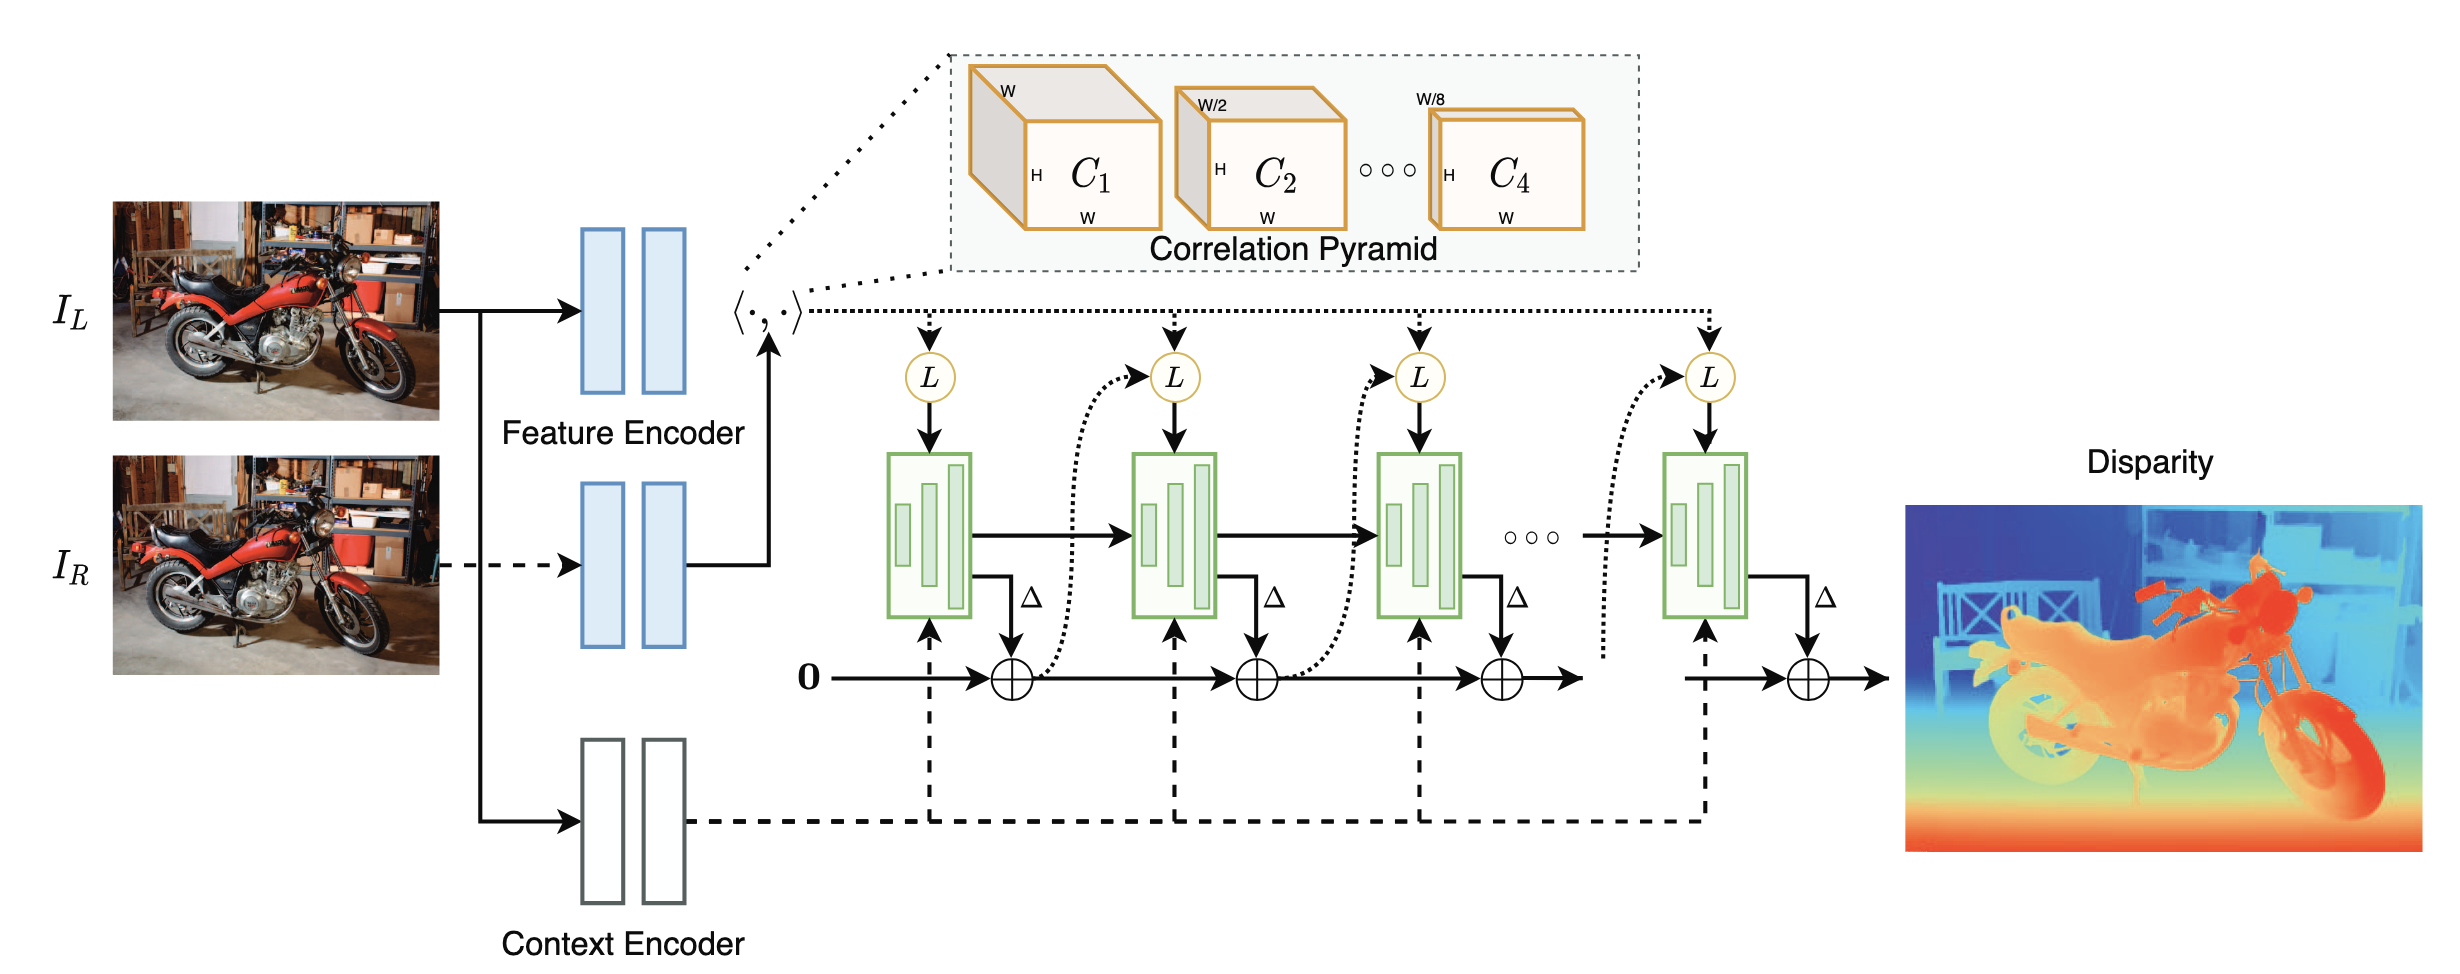
\includegraphics[width=\linewidth]{figures/raft_stereo.png}
	\caption{\bfseries RAFT-Stereo architecture (adapted from \cite{lipson_raft-stereo_2021}).}
	\label{fig:raft_stereo}
\end{figure}

\subsection{Monocular Depth Estimation}
We evaluate the following monocular dense depth estimation models:
\label{sec:monocular_depth_estimation}
\begin{itemize}
	\item \textbf{Depth Anything V2}~\cite{yang_depth_2024}: A transformer-based model trained on a dataset of over 62 million synthetic and pseudo-labeled real images. It is released in variants from 25M to 1.3B parameters for zero-shot relative depth estimation.

	\item \textbf{GLPN}~\cite{kim_global-local_2022}: An architecture that uses a transformer-based encoder to capture global context and a lightweight decoder. A selective feature fusion module combines features from different stages of the encoder.

	\item \textbf{DPT}~\cite{ranftl_vision_2021}: Uses a Vision Transformer (ViT) as its backbone for dense prediction tasks. It processes feature maps at a constant resolution, providing global receptive fields at every stage of the network.

	\item \textbf{Depth Pro}~\cite{bochkovskii_depth_2025}: A model for zero-shot metric depth estimation that uses a multi-scale vision transformer and is designed to operate on high-resolution inputs (e.g., 1536x1536).
\end{itemize}


\subsection{Semantic Segmentation}
We evaluate the following semantic segmentation models:
\label{sec:semantic_segmentation}
\begin{itemize}
	\item \textbf{U-Net}~\cite{ronneberger_u-net_2015}: An encoder-decoder architecture with skip connections that concatenate features from the downsampling path to the upsampling path to retain spatial information.

	\item \textbf{U-Net++}~\cite{zhou_unet_2018}: Modifies the U-Net skip pathways with nested and dense convolutional blocks to reduce the semantic gap between encoder and decoder features.

	\item \textbf{MA-Net}~\cite{fan_ma-net_2020}: Augments an encoder-decoder network with a module that combines position-wise and channel-wise attention to capture contextual dependencies.

	\item \textbf{LinkNet}~\cite{chaurasia_linknet_2017}: A lightweight encoder-decoder network for real-time applications that passes encoder features at each level directly to the corresponding decoder level.

	\item \textbf{FPN}~\cite{lin_feature_2017}: Constructs a multi-scale feature pyramid using a top-down pathway and lateral connections to merge semantic information from deep layers with spatial information from shallow layers.

	\item \textbf{PSPNet}~\cite{zhao_pyramid_2017}: Introduces a pyramid pooling module that applies pooling operations at multiple scales to aggregate global context information.

	\item \textbf{PAN (Path Aggregation Network)}~\cite{li_pyramid_2018}: Augments the top-down feature pyramid with an additional bottom-up pathway to shorten the information path for low-level features.

	\item \textbf{DeepLabV3}~\cite{chen_rethinking_2017}: Uses atrous (dilated) convolutions to control the spatial resolution of feature maps and an Atrous Spatial Pyramid Pooling (ASPP) module to probe features at multiple scales.

	\item \textbf{DeepLabV3+}~\cite{chen_encoder-decoder_2018}: Extends DeepLabV3 by adding a decoder module to refine object boundaries and uses depthwise separable convolutions for computational efficiency.

	\item \textbf{UPerNet}~\cite{xiao_unified_2018}: A unified framework that combines a Feature Pyramid Network (FPN) backbone with a pyramid pooling module to parse features at various scales simultaneously.

	\item \textbf{Segformer}~\cite{xie_segformer_2021}: A transformer-based model using a hierarchical transformer encoder to produce multi-scale features without positional encodings, combined with a lightweight multilayer perceptron (MLP) decoder.

	\item \textbf{DPT}~\cite{ranftl_vision_2021}: Uses a Vision Transformer (ViT) as its backbone, providing global receptive fields at every stage of the feature extraction process for dense prediction tasks.
\end{itemize}

\subsection{3D Gaussian Splatting}
3D Gaussian Splatting (3DGS)~\cite{kerbl_3d_2023} is a rasterization-based method for novel view synthesis that represents a 3D scene with a collection of explicit, optimizable primitives. Unlike implicit representations like NeRF~\cite{mildenhall_nerf_2021}, 3DGS uses thousands to millions of 3D Gaussians to explicitly model the scene's geometry and appearance, as illustrated in \cref{fig:gaussian_splatting}.

Each Gaussian is defined by a set of learnable parameters:
\begin{itemize}
	\item \textbf{Mean:} $\boldsymbol{\mu} \in \mathbb{R}^3$ determines its location in 3D space.
	\item \textbf{Covariance:} $\boldsymbol{\Sigma} \in \mathbb{R}^{3 \times 3}$ defines its shape and orientation. To ensure $\boldsymbol{\Sigma}$ is always a valid positive semi-definite matrix and to allow for intuitive optimization, it is parameterized by a scaling vector $\mathbf{s} \in \mathbb{R}^3$ and a rotation quaternion $\mathbf{q} \in \mathbb{R}^4$.
	      \begin{equation}
		      \boldsymbol{\Sigma} = \mathbf{R} \mathbf{S} \mathbf{S}^\top \mathbf{R}^\top
	      \end{equation}
	      where $\mathbf{R}$ is the rotation matrix derived from $\mathbf{q}$ and $\mathbf{S}$ is a diagonal scaling matrix derived from $\mathbf{s}$.
	\item \textbf{Opacity:} $\alpha \in [0, 1]$ controls the transparency of the Gaussian.
	\item \textbf{Color:} View-dependent color is modeled using Spherical Harmonics (SH) coefficients.
\end{itemize}

\subsubsection{Differentiable Rendering}
To synthesize outputs from a novel viewpoint, the 3D Gaussians are projected onto the 2D image plane, forming elliptical splats. These splats are sorted by depth and composited in a front-to-back order using alpha blending. This differentiable rendering process produces not only the final RGB image ($\hat{I}$), but also a depth map and an accumulation (opacity) map. The rendered image can be directly compared to a ground truth image for gradient-based optimization, while the depth and accumulation maps provide additional supervision or regularization signals as needed.

\subsubsection{Adaptive Densification Strategy}
A key component of the 3DGS training process is the strategy for adaptive densification, which dynamically adjusts the set of Gaussians to efficiently represent the scene. This process is governed by periodic checks that add or remove primitives based on three main heuristics: the magnitude of the positional image-plane gradient, the 3D scale, and the opacity of each Gaussian. The strategy consists of three primary operations: growing, pruning, and opacity reset.

\begin{itemize}
	\item \textbf{Growing (Densification)}:
	      To represent complex regions that are not yet well-reconstructed, new Gaussians are introduced where the image-plane gradients exceed a threshold. This indicates that the optimizer is struggling to place the existing Gaussians correctly. Two methods are used:
	      \begin{itemize}
		      \item Duplication: If a Gaussian has a high gradient and small 3D scale, it is duplicated to add detail in under-reconstructed regions.
		      \item Splitting: If a Gaussian has a high gradient and large 3D scale, it is split into two smaller Gaussians to better capture complex geometry.
	      \end{itemize}

	\item \textbf{Pruning}:
	      To maintain a compact representation and remove artifacts, unnecessary Gaussians are pruned. A Gaussian is removed if it meets certain criteria, such as:
	      \begin{itemize}
		      \item Its opacity $\alpha$ falls below a minimum threshold, rendering it effectively invisible.
		      \item Its 3D scale grows excessively large, which can cause blurry or hazy artifacts.
	      \end{itemize}

	\item \textbf{Opacity Reset}:
	      Periodically during training, the opacities of all Gaussians are reset to a low value. This acts as a regularizer, forcing the model to re-evaluate the importance of each Gaussian. Primitives that are essential to the reconstruction will quickly regain high opacity, while transient or unnecessary ones will fail to do so and be removed in a subsequent pruning phase.
\end{itemize}

\subsubsection{Loss Function}
The total loss $\mathcal{L}_{\text{total}}$ used to train the standard 3DGS model is a weighted sum of a reconstruction loss and a scale regularization term.

The reconstruction loss $\mathcal{L}_{\text{recon}}$ combines the L1 and D-SSIM losses, balanced by a hyperparameter $\lambda_{\text{SSIM}}$:
\begin{equation}
	\mathcal{L}_{\text{recon}} = (1 - \lambda_{\text{SSIM}}) \cdot \|I - \hat{I}\|_1 + \lambda_{\text{SSIM}} \cdot \left(1 - \text{SSIM}(I, \hat{I})\right)
\end{equation}
where $I$ is the ground truth image and $\hat{I}$ is the rendered image.

To prevent the Gaussians from becoming overly stretched, a scale regularization loss $\mathcal{L}_{\text{scale}}$ is applied. For each Gaussian $g$ with a scale vector $\mathbf{s}_g$ out of $N_g$ total Gaussians, this loss penalizes the ratio of its largest to smallest scale component if it exceeds a threshold $\tau_{\text{ratio}}$:
\begin{equation}
	\mathcal{L}_{\text{scale}} = \frac{1}{N_g} \sum_{g=1}^{N_g} \max \left( 0, \frac{\max(\mathbf{s}_g)}{\min(\mathbf{s}_g)} - \tau_{\text{ratio}} \right)
\end{equation}

The final loss is the sum of these two components, with a weighting factor $\lambda_{\text{scale}}$ for the regularization term:
\begin{equation}
	\mathcal{L}_{\text{total}} = \mathcal{L}_{\text{recon}} + \lambda_{\text{scale}}\mathcal{L}_{\text{scale}}
\end{equation}

\begin{figure}[t]
	\centering
	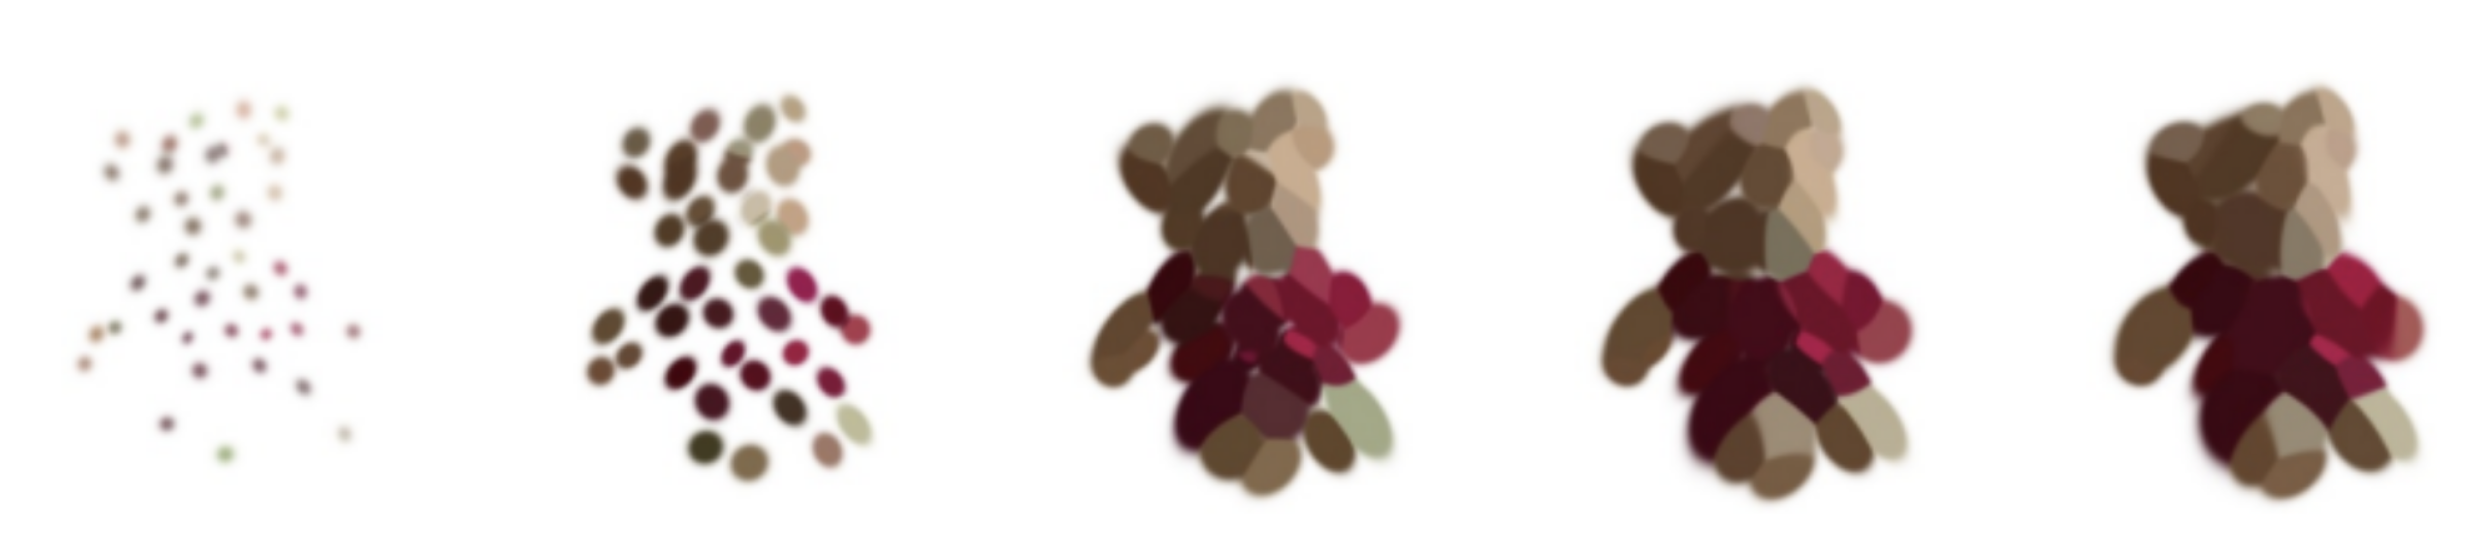
\includegraphics[width=\linewidth]{figures/gaussian_splatting.png}
	\caption{\bfseries 3D Gaussian Splatting (adapted from \cite{dalal_gaussian_2024}).}
	\label{fig:gaussian_splatting}
\end{figure}
